\documentclass{article}

\usepackage{times}
\usepackage{graphicx} % more modern
\usepackage{subfigure} 
\usepackage{natbib}
\usepackage{algorithm}
\usepackage{algorithmic}

\newif\ifsup\supfalse



\usepackage{hyperref}
\newcommand{\theHalgorithm}{\arabic{algorithm}}
\usepackage{icml2016stylefiles/icml2016} 
\usepackage{tikz}
\usepackage{dsfont}
\usepackage{amsmath}
\usepackage{amssymb}
\usepackage{amsthm}



\setlength{\marginparwidth}{10ex}%added by Yifan so that the todos can fit in the margin
\usepackage[obeyFinal]{todonotes}
%\usepackage[disable]{todonotes}

\newcommand{\tinytodo}[2][]{\todo[size=\tiny]{#2}}
%\newcommand{\tinytodo}[2][]{\todo[size=\tiny, #1]{\begin{spacing}{1.0}#2\end{spacing}}}
\newcommand{\todot}[2][]{\tinytodo[color=blue!20, #1]{T: #2}} % Tor
\newcommand{\todof}[2][]{\tinytodo[color=red!20, #1]{F:\@#2}} % Finn
\newcommand{\todom}[2][]{\tinytodo[color=green!20, #1]{M:\@#2}} % Mark


\graphicspath{ {figures/} }
\usetikzlibrary{arrows,positioning} 
\tikzset{
    %Define standard arrow tip
    >=stealth',
    %Define style for boxes
    observed/.style={
           circle,
           rounded corners,
           draw=black, thick,
           minimum width=2.5em,
           minimum height=2.5em,
           font=\footnotesize,
           text centered,
           fill=blue!20!white},
     latent/.style={
           circle,
           rounded corners,
           draw=black, thick, dashed,
           minimum width=.5em,
           minimum height=.5em,
           font=\footnotesize,
           text centered,
           fill=black!10!white
           },
     empty/.style={
           circle,
           rounded corners,
           minimum width=.5em,
           minimum height=.5em,
           font=\footnotesize,
           text centered,
           },
    % Define arrow style
    pil/.style={
           o->,
           thick,
           shorten <=2pt,
           shorten >=2pt,},
    sh/.style={ shade, shading=axis, left color=red, right color=green,
    shading angle=45 }  
}

\newcommand{\defined}{\vcentcolon =}
\newcommand{\rdefined}{=\vcentcolon}
\newcommand{\E}[1]{\mathbb E\left[#1\right]}
\newcommand{\R}{\mathbb R}
\newcommand{\Var}{\operatorname{Var}}
\newcommand{\calF}{\mathcal F}
\newcommand{\sr}[1]{\stackrel{#1}}
\newcommand{\set}[1]{\left\{#1\right\}}
\newcommand{\ind}[1]{\mathds{1}\!\!\set{#1}}
\newcommand{\argmax}{\operatornamewithlimits{arg\,max}}
\newcommand{\argmin}{\operatornamewithlimits{arg\,min}}
\newcommand{\floor}[1]{\left \lfloor {#1} \right\rfloor}
\newcommand{\ceil}[1]{\left \lceil {#1} \right\rceil}
\newcommand{\eqn}[1]{\begin{align}#1\end{align}}
\newcommand{\eq}[1]{\begin{align*}#1\end{align*}}
\newcommand{\Ber}{\operatorname{Bernoulli}}
\renewcommand{\P}[1]{\operatorname{P}\left\{#1\right\}}
\newcommand{\Pri}[1]{\operatorname{P}_i\left\{#1\right\}}
\newcommand{\Prz}[1]{\operatorname{P}_0\left\{#1\right\}}
\newcommand{\bigo}[1]{\mathcal{O}\left( #1 \right)}
\newcommand{\bigotilde}[1]{\tilde{\mathcal{O}}\left( #1 \right)}
\newcommand{\bigtheta}[1]{\Theta\left( #1 \right)}
\newcommand{\bigthetatilde}[1]{\tilde{\Theta}\left( #1 \right)}
\newcommand{\bigomega}[1]{\Omega\left( #1 \right)}
\newcommand{\KL}{\operatorname{KL}}
\newcommand{\simpleregret}{R_T}
\newcommand{\Pij}[1]{\operatorname{P}_{ij}\!\left\{#1\right\}}
\newcommand{\Pkl}[1]{\operatorname{P}_{kl}\!\left\{#1\right\}}
\newcommand{\Q}[1]{\operatorname{Q}\left\{#1\right\}}
\newcommand{\EE}{\mathbb E}
\newcommand{\Pn}[2]{\operatorname{P}_{#1}\left\{#2\right\}}
\newcommand{\parents}[1]{\operatorname{Pa}_{#1}}
\newcommand{\actions}{\mathcal{A}}
\newcommand{\calA}{\mathcal A}

\newcommand{\etc}{\textit{etc}}
\newcommand{\ie}{\textit{i.e.}}
\newcommand{\eg}{\textit{e.g.}}

\theoremstyle{plain}
\newtheorem{theorem}{Theorem}
\newtheorem{proposition}[theorem]{Proposition}
\newtheorem{lemma}[theorem]{Lemma}
\newtheorem{corollary}[theorem]{Corollary}
\theoremstyle{definition}
\newtheorem{definition}[theorem]{Definition}
\newtheorem{assumption}[theorem]{Assumption}
\newtheorem{remark}[theorem]{Remark}
\newtheorem{example}[theorem]{Example}
\let\temp\epsilon
\let\epsilon\varepsilon


% The \icmltitle you define below is probably too long as a header.
% Therefore, a short form for the running title is supplied here:
\icmltitlerunning{Causal Bandits}

\begin{document} 

\twocolumn[
\icmltitle{Causal Bandits: Learning Good Interventions via Causal Inference}
% ALTERNATIVES:
% - Causal Bandits: Sequential Decision Making with Causal Models

% It is OKAY to include author information, even for blind
% submissions: the style file will automatically remove it for you
% unless you've provided the [accepted] option to the icml2015
% package.
\icmlauthor{Your Name}{email@yourdomain.edu}
\icmladdress{Your Fantastic Institute,
            314159 Pi St., Palo Alto, CA 94306 USA}
\icmlauthor{Your CoAuthor's Name}{email@coauthordomain.edu}
\icmladdress{Their Fantastic Institute,
            27182 Exp St., Toronto, ON M6H 2T1 CANADA}

% You may provide any keywords that you 
% find helpful for describing your paper; these are used to populate 
% the "keywords" metadata in the PDF but will not be shown in the document
\icmlkeywords{causal,bandit}

\vskip 0.3in
]

\begin{abstract} 
We study the problem of using causal models to improve the rate at which good interventions can be learned online in a stochastic environment. 
Our formalism combines multi-arm bandits and causal inference to model a novel type of bandit feedback that is not exploited by existing approaches.
We propose a new algorithm that exploits the causal feedback and prove a bound on its simple regret that is strictly better (in all quantities) 
than algorithms that do not use the additional causal information.
\end{abstract} 

%%%%%%%%%%%%%%%%%%%%%%%%%%%%%%%%%%%%%%%%%%%%%%%%%
% INTRODUCTION
%%%%%%%%%%%%%%%%%%%%%%%%%%%%%%%%%%%%%%%%%%%%%%%%%
\section{Introduction}
\label{sec:intro}
Medical drug testing, policy setting, and other scientific processes are commonly framed and analysed in the language of sequential experimental design and, in special cases, as bandit problems~\citep{Robbins1952,Chernoff1959}. 
In this framework, single actions (\eg, experiments or interventions) from a pre-determined set are repeatedly performed in 
order to evaluate their effectiveness via feedback from a single, real-valued reward signal.
We propose a generalisation of the standard model by assuming that, in additional to the reward signal, the learner observes the values of a number of covariates 
drawn from a probabilistic causal model~\citep{Pearl2000}.
Causal models are commonly used in disciplines where explicit experimentation may be difficult such as social science, demography and economics.
For example, when predicting the effect of changes to childcare subsidies on workforce participation, or school choice on grades. 
Results from causal inference relate observational distributions to interventional ones, allowing the outcome of an intervention to be predicted without
explicitly performing it.
By exploiting the causal information we show, theoretically and empirically, how non-interventional observations can be used to improve the rate at 
which high-reward actions can be identified.

The type of problem we are concerned with is best illustrated with an example. 
Consider a farmer wishing to optimise the yield of her crop. 
She knows that crop yield is only affected by temperature, a particular soil nutrient, and moisture level but the precise effect of their combination is unknown.
In each season the farmer has enough time and money to intervene and control at most one of these variables:
deploying shade or heat lamps will set the temperature to be low or high; the nutrient can be added or removed a through a choice of fertilizer; and irrigation or rain-proof covers will keep the soil wet or dry.
When not intervened upon, the temperature, soil, and moisture vary naturally from season to season due to weather conditions and these are all observed along with the final crop yield at the end of each season.
How might the farmer best experiment to identify the single, highest yielding intervention in a limited number of seasons?
%without sacrificing too much crop yield (relative to always choosing the best intervention) in the process?


\subsection{Contributions}

This paper takes the first step towards formalising and solving problems such as the one above. 
In \S\ref{sec:defs} we formally introduce \emph{causal bandit problems} in which interventions are treated as arms in a bandit problem but their influence on the reward --- along with any other observations --- is assumed to conform to a known causal graph. 
We show that our causal bandit framework subsumes the classical bandits (no additional observations) and contextual stochastic bandit problems (observations are revealed before an intervention is chosen) before focusing on the case where, like the above example, observations occur \emph{after} each intervention is made.

We focus on the simple regret, which measures the difference between the return of the optimal action and that of the action chosen by the algorithm after $T$ rounds.
In \S\ref{sec:simple-regret} we analyse a specific family of causal bandit problems that we call \emph{parallel bandit} problems in which $N$ factors affect the reward independently and there are $2N$ possible interventions.
We propose a simple causal best arm identification algorithm (Algorithm~\ref{alg:simple}) for this problem and show that up to logarithmic factors it enjoys minimax optimal
simple regret guarantees of $\tilde\Theta(\sqrt{m/T})$ where $m$ depends on the causal model and may be much smaller than $N$.
In contrast, existing best arm identification algorithms suffer $\Omega(\sqrt{N/T})$ simple regret.
This shows theoretically the value of our framework over the traditional bandit problem. 
Experiments in \S\ref{sec:experiments} further demonstrate the value of causal models in this framework.

In the general casual bandit problem interventions and observations may have a complex relationship. 
In \S\ref{sec:simple-regret-general} we propose a novel algorithm inspired by importance-sampling that a) enjoys sub-linear regret equivalent to the optimal rate in the parallel bandit setting and b) captures many of the intricacies of sharing information in a causal graph in the general case.
As in the parallel bandit case, the regret guarantee is often significantly better than $O(\sqrt{N/T})$ and never worse, where $N$ is the number of available interventions.



\subsection{Related Work}

As alluded to above, causal bandit problems with $N$ possible interventions can be treated as a classical $N$-armed bandit problem by simply ignoring the causal model and extra observations that are revealed each round.
In the farming example, the farmer could treat the six possible interventions are arms, ignore the observations of the non-intervened variables, and apply an existing best-arm identificaion algorithm~\citep{Jamieson2013} with well understood simple regret guarantees.
However, as we show in \S\ref{sec:simple-regret}, this approach ignores the extra information available in the non-intervened variables and subsequently yields sub-optimal performance.

A well-studied class of bandit problems with side information are ``contextual bandits''~\cite{Langford2008,Agarwal2014}.
Our framework bears a superficial similarity to contextual bandit problems since the extra observations on non-intervened variables might be viewed as context for selecting an intervention. 
However, a crucial difference is that in our model the extra observations are only revealed \emph{after} selecting an intervention and hence cannot be used as context.
% We discuss the relationship between causal and contextual bandits further in \S\ref{sec:defs} and leave their combination as future work.

There have been several proposals for bandit problems where extra feedback is received after an action is taken.
\citet{Alon2015}, \citet{Kocak2014} and \citet{wu2015online} consider very general models where rewards on unplayed actions are revealed according to a feedback graph.
As we discuss in \S\ref{sec:discussion}, the problem they consider shares some similarity with ours however their results are for cumulative regret and thus cannot be used to guarantee low simple regret~\citep{Bubeck2009}.
% Even in the case of cumulative regret we show that an application of their results to the parallel bandit problem with $N$ variables yields a $\bigo{\sqrt{NT}}$ bound.
\citet{Yu2009} consider bandit problems where a learner chooses an arm to play as well as set of arms to observe rewards for in a stochastic setting where the reward distributions can change infrequently and the aim is to minimize cumulative regret.
They use extra observations to detect changes whereas we assume fixed reward distributions and use extra observations to improve arm selection.
\citet{Avner2012} analyse bandit problems where the choice of arm to pull and arm to receive feedback on are decoupled. 
The main difference from our present work is our focus on simple regret and exploitation of the more complex information related rewarding via the causal graph.
To the best of our knowledge, our paper is the first to analyse simple regret in bandit problems with extra post-action feedback.


% Partial monitoring is a very general framework for for decoupling the feedback from the action and reward. It can be used to classify problems into one of four categories, trivial with no regret, easy with $R_T = \bigthetatilde{\sqrt{T}}$ , hard with $R_T = \bigtheta{T^{2/3}}$ and hopeless with $R_T = \bigomega{T}$ \cite{Bartok2014}. Partial monitoring algorithms yield results that are optimal with respect the horizon $T$ but not other parameters, such as $K$, which is the key focus of incorporating causal structure. 

Two pieces of recent work also consider using causal models in bandit problems.
\citet{Bareinboim2015} also use causal inference to improve the chance of choosing an optimal arm. Their work differs from ours in two key ways. Firstly, their focus is on correcting the effects of unobserved confounding variables whereas we assume all variables are observable. Secondly, they do not assume their learning algorithm has access to a causal graph and instead use a form of contextual randomization to improve reward estimates in a Thompson sampling-style algorithm. \citet{Ortega2014thompson} present an analysis and extension of Thompson sampling assuming actions are causal interventions. Their focus is on causal induction (\ie, learning an unknown causal model) instead of exploiting a known causal model. Neither work provides a regret analysis. 
Combining their handling of unobserved variables and causal induction with our analysis is left as future work.
% Key to Elias' paper is: observing the action an agent would take if it were allowed to make its natural choice can provide some information about hidden confounders that influence both the reward and the choice of action. Therefore, incorporating an agents natural choice as context may outperform a standard bandit that does not use that context. (Note: even in the presence of hidden confounders, including the agents natural choice as context only may improve the results. It is easy to come up with a counter example in which it does not).




%%%%%%%%%%%%%%%%%%%%%%%%%%%%%%%%%%%%%%%%%%%%%%%%%
% PROBLEM SETUP
%%%%%%%%%%%%%%%%%%%%%%%%%%%%%%%%%%%%%%%%%%%%%%%%%
\section{Problem Setup}
\label{sec:defs}
\newcommand{\bernoulli}{\operatorname{Bernoulli}}
\newcommand{\dirac}{\operatorname{Dirac}}
\renewcommand{\vec}[1]{\boldsymbol{#1}}

We now introduce a novel class of stochastic sequential decision problems which we call \emph{causal bandit problems}. 
In these problems, rewards are given for repeated interventions on a fixed causal model~\cite{Pearl2000}. 
Following the terminology and notation in~\cite{Koller2009}, a \emph{causal model} is given by a directed acyclic graph $\mathcal{G}$ over a set of random variables $\mathcal{X} = \{ X_1, \ldots, X_N \}$ and a joint distribution $\mathrm{P}$ over $\mathcal{X}$ that factorises over $\mathcal{G}$.
We will assume each variable only takes on a finite number of distinct values.
An edge from variable $X_i$ to $X_j$ is interpreted to mean that a change in the value of $X_i$ may directly cause a change to the value of $X_j$.
The \emph{parents} of a variable $X_i$, denoted $\parents{X_i}$ or just $\parents{i}$, is the set of all variables $X_j$ such that there is an edge from $X_j$ to $X_i$ in $\mathcal{G}$.
An \emph{intervention (of size $n$)}, denoted $do(\vec{X}=\vec{x})$, assigns the values $\vec{x}=\{x_1, \ldots, x_n\}$ to the corresponding variables $\vec{X}=\{X_1, \ldots, X_n\} \subset \mathcal{X}$ with the empty intervention (where no variable is set) denoted $do()$.
The intervention also ``mutilates'' the graph $\mathcal{G}$ by removing all edges from the parents of $X_i$ to $X_i$ for each $X_i \in \vec{X}$. 
The resulting graph defines a probability distribution $\P{\vec{X}^c | do(\vec{X}=\vec{x})}$ over $\vec{X}^c := \mathcal{X} - \vec{X}$. 
Details can be found in Chapter 21 of~\cite{Koller2009}.

A learner for a casual bandit problem is given the casual model's graph $\mathcal{G}$ and a set of \emph{allowed interventions} $\mathcal{A}$.
One variable $Y \in \mathcal{X}$ is designated as the \emph{reward variable} and takes on values in $\{0, 1\}$.
We denote the expected reward for the intervention $a = do(\vec{X} = \vec{x})$ by $\mu_{a} := \E{Y | do(\vec{X} = \vec{x})}$ and 
the optimal expected reward by $\mu^* := \max_{a\in\actions} \mu_{a}$. 

The game proceeds over $T$ rounds.
In round $t$, the learner \emph{intervenes} by choosing $a_t = do(\vec{X}_t = \vec{x}_t) \in \mathcal{A}$ based on previous observations. 
It then \emph{observes} sampled values for all non-intervened variables $\vec{X}^c_t$ drawn from $\P{\vec{X}^c_t | do(\vec{X}_t = \vec{x}_t)}$, 
including the \emph{reward} $Y_t \in \{0,1\}$. 
After $T$ observations the learner outputs an estimate of the optimal action $\hat a^*_T$.

The objective of the learner is to minimise the simple regret
\begin{equation}
\label{eq:regret-simple}
	\simpleregret = \mu^* - \E{\mu_{\hat a^*_T}}.
\end{equation}
This is sometimes refered to as a ``pure exploration''~\citep{Bubeck2009} or ``best-arm identification'' problem~\citep{Gabillon2012} and
is most appropriate when the learner has a fixed learning budget after which its policy will be fixed indefintely. 

Although we will focus on the intervene-then-observe ordering of events within each round, other scenarios are possible. 
If the non-intervened variables are observed before an intervention is selected our framework 
reduces to stochastic contextual bandits, which are already reasonably well understood~\citep{Agarwal2014}. 
Even if no observations are made during the rounds, the causal model may still allow offline pruning of the set of 
allowable interventions thereby reducing the complexity.


We note that classical $K$-armed stochastic bandit problem can be recovered in our framework by considering a simple causal model with one 
edge connecting a single variable $X$ that can take on $K$ values to a reward variable $Y \in \set{0,1}$ where $\P{Y = 1|X} = r(X)$ for some 
arbitrary but unknown, real-valued function $r$. The set of allowed interventions in this case is $\mathcal{A} = \{ do(X = k) \colon k \in \{1, \ldots, K\}\}$.
Conversely, any causal bandit problem can reduced to a classical stochastic $|\mathcal{A}|$-armed bandit problem by 
treating each possible intervention as an arm and ignoring all sampled values for the observed variables except for the reward.
Intuitively though, one would expect to perform better by making use of the extra observations.



\iffalse
\subsection{Exploiting the Causal Model}

From a causal perspective the key insight is that the assumed causal structure implies that
the law of $Y_t$ given we intervene to set $X_{t,i} = j$ is the same as the law of $Y_t$ conditioned
on $X_{t,i} = j$. Formally,
\eqn {
\label{eq:observe}
\P{Y_t \leq y|do(X_{t,i} = j)} = \P{Y_t \leq y|do(),X_{t,i} = j}\,.
}
This follows from application of the do-calculus \cite{Pearl2000} to the causal graph for the parallel bandits problem (Figure \ref{fig:causalStructure}). It is not the case in general. 
For example if there was a variable $X'$ that caused both $X_{t,i}$ and $Y$ (or $X_{t,i}$ and any other variable $X_{t,l}$),that would introduce a backdoor path from $X_{t,i} \rightarrow Y_t$ and we would have to condition on $X'$ to derive the interventional distribution of $Y_t$ from the observational one.

This enables us to estimate the rewards for multiple interventions simultaneously by observing the values taken by the variables when we select the $do()$ action. Unfortunately interventions that occur with low probability ($\P{X_{t,i} = j}$ is small) suffer from a high approximation error and need to be explored separately, by explicitly making the intervention. 

To exploit the causal structure we must optimally balance the collection of observational data against making interventions to learn about low probability events. The problem is more challenging because the probabilities $P(X_i=j)$ are unknown and must also be estimated.

\begin{definition}
Let $V_{ij} = \frac{1}{P(X_i = j)}$, for $i \in \set{1...N}$ and $j \in {0,1}$. 
Define 
\eqn{
\label{def:m}
m(\boldsymbol{V}) = \min \set{m: \sum_{ij} \ind{V_{ij} \geq m} = m}\,.
}
\end{definition}

\fi


%%%%%%%%%%%%%%%%%%%%%%%%%%%%%%%%%%%%%%%%%%%%%%%%%
% UPPER BOUND ON SIMPLE REGRET
%%%%%%%%%%%%%%%%%%%%%%%%%%%%%%%%%%%%%%%%%%%%%%%%%
\section{Regret Bounds for Parallel Bandit}
\label{sec:simple-regret}



In this section we propose and analyse an algorithm for achieving the optimal regret in a natural special 
case of the causal bandit problem which we call the {\it parallel bandit}.
It is simple enough to admit a thorough analysis but rich enough to model the type of problem discussed in \S\ref{sec:intro}, including the farming example. 
It also suffices to witness the regret gap between algorithms that make use of causal models and those which do not.

The causal model for this class of problems has $N$ binary variables $\{ X_1, \ldots, X_N \}$ where each $X_i \in \{0,1\}$ are independent causes of a 
reward variable $Y \in \set{0,1}$, as shown in Figure~\ref{fig:causalStructure}.
All variables are observable and the set of allowable actions are all size 0 and size 1 interventions: 
\eq{
	\mathcal{A} = \set{do()} \cup \set{ do(X_i = j) \colon 1 \leq i \leq N \text{ and } j \in \set{0,1}}\,.
}
In the farming example from the introduction, $X_1$ might represent temperature (\eg, $X_1=0$ for low and $X_1=1$ for high). 
The interventions $do(X_1 = 0)$ and $do(X_1 = 1)$ indicate the use of shades or heat lamps to keep the temperature low or high, respectively.

\begin{wrapfigure}[11]{r}{0.5\textwidth}
  \begin{center}
    \begin{tikzpicture}[->,>=stealth',shorten >=1pt,auto,node distance=1cm,
  thick,main node/.style={observed}, hidden/.style={empty}]

 %nodes
\node[main node](1){$X_{1}$};
\node[main node, right=of 1](2){$X_{2}$};
\node[hidden, right=of 2](3){$...$};
\node[main node, right=of 3](4){$X_{N}$};
\node[main node, below right=of 2](5){Y};
 \path[every node/.style={font=\sffamily\small}]
    (1) edge (5)
    	(2) edge (5)
    (4) edge (5);
	
\end{tikzpicture}
  \end{center}
  \caption{Causal model for the parallel bandits problem.\label{fig:causalStructure}}
\end{wrapfigure}

In each round the learner either purely observes by selecting $do()$ or chooses a single variable to intervene on and the value to set it to. 
The remainder of the variables are simultaneously set by independently biased coin flips. 
The value of all variables are then used to determine the distribution of rewards for that round.
Formally, when not intervened upon we assume that each $X_i \sim \bernoulli(q_i)$ where $\vec{q} = (q_1, \ldots, q_N) \in [0,1]^N$ so that $q_i = \P{X_i = 1}$.
%\todom{Should $Y$ be 0-1 valued or real everywhere?} YES!
The value of the reward variable is distributed as $\P{Y = 1|\vec{X}} = r(\vec{X})$ where 
$r : \{0,1\}^N \to [0,1]$ is an arbitrary, fixed, and unknown function. 
In the farming example, this choice of $Y$ models the success or failure of a seasons crop, which depends stochastically on the various environment variables.
Note that the expected reward of the optimal intervention is at least as large as the expected reward for doing nothing.

%\todom{$i,j$ notation to $a \in \actions$}
%In our analysis below, we will often use the pair $(i,j)$ for $i \in \{1, \ldots, N\}$ and $j \in \{0,1\}$ as a shorthand for the intervention $do(X_i = j)$.
%We will also make use of the expansion of the expected reward for $do(X_i = j)$:
%\eq{
%\mu_{i,j} 
%&= \E{r(X)|do(X_i = j)} \\
%&= \sum_{\boldsymbol{x} \in \set{0,1}^N : x_i = j} r(\boldsymbol{x})  \prod_{k \neq i} q_k^{x_k} (1 - q_k)^{1-x_k}\,.  
%}
%The sum and product use the restrictions $x_i = j$ and $k \ne i$ because the intervention forces $X_i = j$ with probability 1.
%The optimal intervention is denoted $(i^*,j^*) = \argmax_{i,j} \mu_{i,j}$ and the corresponding optimal reward is $\mu^* = \mu_{i^*,j^*}$. 



\subsection{The Parallel Bandit Algorithm}
\label{sub:par-bandit-alg}

The algorithm operates as follows. For the first $T/2$ rounds it chooses $do()$ to collect observational data.
The fact that the only link from each $X_1,\ldots,X_N$ to $Y$ is a direct, causal one means that $\P{Y|do(X_i=j)}=\P{Y|X_i=j}$. Thus we can create good estimators of the returns of those actions $do(X_i = j)$ for which $\P{X_i = j}$ is large. 
These are the interventions that are easily estimated ``passively'' (\ie, without playing them explicitly). 
Those actions where $\P{X_i = j}$ is small may not be observed (often) in the first $T/2$ rounds, so
the estimates of the returns of these actions from the first $T/2$ samples could be quite poor. For the remaining $T/2$ rounds
the algorithm makes interventions on the actions $a = do(X_i = j)$ for which $\P{X_i = j}$ is small. The precise allocation is
carefully chosen to minimise the worst-case simple regret. 
The difficulty of the problem depends on $\vec{q}$ and, in particular, how many of the variables have an infrequently occurring value (\ie, small $q_i$ or $1-q_i$). 
Let $I_1 = \emptyset$ and for $\tau \in [0,1)$ let $I_\tau = \set{ i : \min\set{q_i, 1-q_i} \leq \tau}$.
Define
\eqn{
\label{eq:m-simple}
m(\vec{q}) = \max \set{ d : |I_{\frac{1}{d}}| \leq d}\,.
% m(\vec{q}) = \max \set{i : \sum_{k=1}^N \ind{\min\set{q_k, \,1 - q_k} \leq 1/i} \leq i}\,.
}
This captures a trade off between identifying the low probability variables and not having too many of them.
When $\vec{q} = (\frac{1}{2}, \ldots, \frac{1}{2})$ we have $m(\vec{q}) = 1$ and when $\vec{q} = (0, \ldots, 0)$ we have $m(\vec{q}) = N$, the number of variables.

To identify a high-reward intervention, Algorithm~\ref{alg:simple} break $T$ rounds into halves. 
In the first half, the non-interventional action $do()$ is played and the rewards observed.
These are used to estimate the occurrance probabilities $\vec{q}$ and the value of $m(\vec{q})$.
The remainder of the rounds are then evenly split to estimate the infrequently observed interventions, as determined by the estimate for $m(\vec{q})$.
Although very simple, the following two theorems show that this algorithm is effectively optimal.

\begin{wrapfigure}[22]{r}{0.6\textwidth}
\vspace{-10pt}
\begin{minipage}{.6\textwidth}
\begin{algorithm}[H]
\caption{Parallel Bandit Algorithm}\label{alg:simple}
\begin{algorithmic}[1]
\STATE {\bf Input:} Total rounds $T$ and $N$.
\FOR{$t \in 1,\ldots,T / 2$}
\STATE Perform empty intervention $do()$
\STATE Observe $\vec{X}_t$ and $Y_t$
\ENDFOR
\FOR{$a = do(X_i = x) \in \actions$}
\STATE Count times $X_i = x$ seen: $T_a = \sum_{t=1}^{T/2} \ind{X_{t,i} = x}$
\STATE Estimate reward: $\hat{\mu}_a = \frac{1}{T_a} \sum_{t=1}^{T/2} \ind{X_{t,i} = x} Y_t$ \\[0.2cm]
\STATE Estimate probabilities: $\hat{p}_a = \frac{2 T_a}{T}$,\,\, $\hat q_i = \hat p_{do(X_i = 1)}$
\ENDFOR
\STATE Compute $\hat{m} = m(\vec{\hat q})$ and $A = \set{a \in \actions \colon \hat{p}_a \leq \frac{1}{\hat m}}$.
\STATE Let $T_A := \frac{T}{2 |A|}$ be times to sample each $a\in A$.
\FOR{$a = do(X_i = x) \in A$}
\FOR{$t \in 1,\ldots,T_A$}
\STATE Intervene with $a$ and observe $Y_t$
\ENDFOR
\STATE Re-estimate $\hat{\mu}_a = \frac{1}{T_A} \sum_{t=1}^{T_A} Y_t$
\ENDFOR
\RETURN estimated optimal $\hat{a}^*_T \in \argmax_{a\in\actions} \hat{\mu}_a$
\end{algorithmic}
\end{algorithm}
\end{minipage}
\end{wrapfigure}

\begin{theorem}\label{thm:uq-simple}
Algorithm \ref{alg:simple} satisfies
\eq{
\simpleregret \in \bigo{\sqrt{\frac{m(\vec{q})}{T}\log\left(\frac{NT}{m}\right)}}\,.
}
\end{theorem}

Note that algorithms designed for finite-armed bandits would explore interventions more uniformly and achieve a regret of $\Omega(\sqrt{N/T})$.
Since $m$ is typically much smaller than $N$ we anticipate that the new algorithm will significantly outperform classical bandit algorithms in
this setting.
We prove a lower bound on the simple regret that matches up to logarithmic factors the upper bound given in Theorem \ref{thm:uq-simple}.

\begin{theorem}\label{thm:lower}
For all $T$, $\vec{q}$ and all strategies, there exists a reward function such that
\eq{
\simpleregret 
\in \Omega\left(\sqrt{\frac{m(\vec{q})}{T}}\right)\,.
}
\end{theorem}

\ifsup
The proofs of Theorems \ref{thm:uq-simple} and \ref{thm:lower} may be found in Sections \ref{sec:thm:uq-simple} and \ref{sec:thm:lower} respectively.
\else
The proofs of Theorems \ref{thm:uq-simple} and \ref{thm:lower} follow by carefully analysing the concentration
of $\hat p_a$ and $\hat m$ about their true values and may be found in the supplementary material.
\fi






%%%%%%%%%%%%%%%%%%%%%%%%%%%%%%%%%%%%%%%%%%%%%%%%%
% UPPER BOUND ON SIMPLE REGRET GENERAL CASE
%%%%%%%%%%%%%%%%%%%%%%%%%%%%%%%%%%%%%%%%%%%%%%%%%
\section{Regret Bounds for General Graphs}
\label{sec:simple-regret-general}

\newcommand{\calP}{\mathcal P}
\newcommand{\x}{\boldsymbol{x}}

We now consider single variable interventions on general causal graphs over variables $\boldsymbol{V}$. Let $Y \in \set{0,1}$ be the target variable and $\boldsymbol{X} = V/\set{Y \cup Desendants(Y)}$. 

If all the variables in $\boldsymbol{X}$ are observable, we can compute the distribution $P(Y,\boldsymbol{X}|do(X_i = j)$ for any intervention $i,j$ via the truncated product formula \cite{Pearl2000} 3.11

\eq {
\P{\boldsymbol{x},y|do(X_i = j)} = 
\begin{cases}
\frac{\P{\boldsymbol{x},y}}{\P{x_i=j|\calP_i(\boldsymbol{x})}} & \text{if} x_i = j  \\
0 & \text{otherwise}
\end{cases}
} 

Where $\calP_i : \set{0,1}^N \to \set{0,1}^{N_i}$ is the
projection that selections the $N_i$ parents of variable $i$. 

Since estimating $\P{Y|do(X_i=j)}$ from observational data requires conditioning on the parents of $X_i$, the variance of our estimators depends on $\P{X_i=j|\calP_i}$, rather than simply being a function of the number of times we observe $X_i=j$ as in the parallel bandit case. For example consider the graph in Figure \ref{fig:causalStructure_confounded}. In this model 
$P(Y|do(X_i = j) = \sum_z P(Y|X_i = j,Z)P(Z)$. Let $P(z=1)=.5$, $P(X_i = 1|z = 1) = 1$, and $P(X_i = 0|z = 0) = 1$ then $P(X_i = 1) = .5$ but we will be unable to estimate $P(Y|do(X_i = 1))$ as we will never get any data for the term $P(Y|X_i = 1, Z = 0)$.

\begin{figure}[h]
\centering
\caption{Causal model for the confounded parallel bandits problem}.\label{fig:causalStructure_confounded}
\begin{tikzpicture}[->,>=stealth',shorten >=1pt,auto,node distance=1cm,
  thick,main node/.style={observed}, hidden/.style={empty}]

 %nodes

\node[main node](1){$X_{1}$};
\node[main node, right=of 1](2){$X_{2}$};
\node[hidden, right=of 2](3){$...$};
\node[main node, right=of 3](4){$X_{N}$};
\node[main node, below right=of 2](5){Y};
\node[main node, above=of 3](6){$Z$};
 \path[every node/.style={font=\sffamily\small}]
    (1) edge (5)
    	(2) edge (5)
    (4) edge (5)
    (6) edge (1) edge (2) edge(4);
	
\end{tikzpicture}
\end{figure} 

For general models, it is also insufficient to only trade off learning about multiple actions by observing against learning individual actions by explicitly playing them. We can also learn about the reward for intervening on one variable from rounds in which we actually set a different variable.

\eqn {
\label{eq:estimation_transfer}
P(Y_t|do(X_{t,i} = j))= & \nonumber \\
 \sum_{j'}  P(Y_t|do(X_{t,l} & = j'),X_{t,i} = j)P(X_{t,l} = j')
}

Consider the graph in Figure \ref{fig:causalchain}, where each variable deterministically takes the value of its parent,$X_k = X_{k-1}$ for $k\in {N...2}$ and $\P{X_1} = 0$. We can learn the reward for all the arms $do(X_i = 1)$ simultaneously by selecting $do(X_1 = 1)$. If we only considered information transfer from one action to another for the case of the $do()$ action, we would have to explicitly play each of these arms individually to estimate their rewards. 

\begin{figure}[h]
\centering
\caption{A causal chain graph}.
\label{fig:causalchain}
\begin{tikzpicture}[->,>=stealth',shorten >=1pt,auto,node distance=1cm,
  thick,main node/.style={observed}, hidden/.style={empty}]

 %nodes
\node[main node](1){$X_{1}$};
\node[main node, right=of 1](2){$X_{2}$};
\node[hidden, right=of 2](3){$...$};
\node[main node, right=of 3](4){$X_{N}$};
\node[main node, right=of 4](5){Y};
 \path[every node/.style={font=\sffamily\small}]
    (1) edge (2)
    	(2) edge (3)
    (3) edge (4)
    (4) edge (5);
\end{tikzpicture}
\end{figure} 

\todof{From here onwards needs to be replaced by truncated importance sampling version}

Let $r(x) = \P{Y = 1|X = x}$. Then

\eq {
\mu_{ij} = P(Y = 1|do(X_i = j)) = \sum_{\x:x_i=j} \P{\boldsymbol{X}|do(X_i=j)}r(x)
}


We wish to devise an estimator for $\mu_{ij}$ using $X$ and $Y$ without
intervening to set $X_i = j$. A natural choice is the importance weighted estimator

\eq{
Z_{ij} 
&= \frac{Y \ind{X_i = j}}{\P{X_i = j|\calP_i(X)}}\,. 
}

Checking:
\eq{
&\E{Z_{ij}} 
= \sum_x \frac{\P{X = x} r(x) \P{X = x | do(X_i = j)}}{\P{X = x}} \\
&= \P{Y = 1| do(X_i = j)} \,. 
}
The variance of $Z_{ij}$ may also be bounded
\eq{
&\Var[Z_{ij}]
\leq \E{Z_{ij}^2} \\
&\leq \sum_x \P{X = x} \left(\frac{\ind{X_i = j}}{\P{X_i = j|\calP_i(X) = \calP_i(x)}}\right)^2 \\
&= \E{\frac{1}{\P{X_i = j|\calP_i(X)}}} \\
&= V_{ij}\,.
}
In the general graph setting the dimension $m$ has a slightly different definition.
\eq{
m = \min\set{m : \sum_{ij} \ind{V_{ij} \leq 1/m} = m}\,.
}

\todof{I think the above should be}

\eq {
m = \min \set{m: \sum_{ij} \ind{V_{ij} \geq m} = m}\,.
}

That is, $m$ should be chosen such that the size of the set variances greater than $m$ is $m$. This ensures all the variances of the remaining arms are smaller than $m$. This definition would also seem equivalent to sorting the variances such that $V^{(0)} \geq V^{(1)} ... \geq V^{(2N)}$ and then defining $m = \min m: V^{(m)} \leq m$ which is in turn equivalent to the definition in terms of $q$ for parallel bandits. 

\begin{algorithm}[H]
\caption{General Algorithm}
\begin{algorithmic}
\STATE {\bf Input:} $N$, $\mathcal P$
\STATE Compute $m$:
\eq{
m = \min\set{m : \sum_{ij} \ind{V_{ij} \leq 1/m} = m}
}
\STATE Collect $T/2$ observational samples and estimate $\hat \mu_{ij}$:
\eq{
\hat \mu_{ij} = \sum_{t=1}^{T/2} \frac{Y_t \ind{X_{t,i} = j}}{\P{X_{t,i} = j | \mathcal P_i(X_t)}}
}
\FOR{$i \in \set{1,\ldots,m}$}
\STATE For each $i,j $ with $V_{ij} < 1/m$ take action $do(X_i = j)$ for $T/(2m)$ samples $Y^{(ij)}_1,\ldots,Y^{(ij)}_{T/2m}$
\STATE Update estimate:
\eq{
\eta &= \frac{V_{ij}}{V_{ij} + m} \\
\hat \mu_{ij} &= \eta \left(\frac{2m}{T} \sum_{t=1}^{T/(2m)} Y^{(ij)}_t\right) + (1 - \eta) \hat \mu_{ij}
}
\ENDFOR
\STATE Choose $do(X_i = j)$ for $ij = \argmax_{ij} \hat \mu_{ij}$
\end{algorithmic}
\end{algorithm}






 


%%%%%%%%%%%%%%%%%%%%%%%%%%%%%%%%%%%%%%%%%%%%%%%%%
% EXPERIMENTS
%%%%%%%%%%%%%%%%%%%%%%%%%%%%%%%%%%%%%%%%%%%%%%%%%
\section{Experiments}
\label{sec:experiments}
In all experiments, the reward is generated according to:
\eq{
Y_t \sim \begin{cases}
\bernoulli(.5+\epsilon) & \text{if } X_1 = 1 \\
\bernoulli(\frac{.5-(.5+\epsilon)q_1}{1-q_1}) & \text{otherwise}\,.
\end{cases}
}

With $\epsilon \in (0,.5)$. This ensures that 
\eq {
\P{Y|do(X_i = j)} = \begin{cases}
.5+\epsilon & \text{if } (i,j)=(1,1) \\
\frac{.5-(.5+\epsilon)q_1}{1-q_1} & \text{if } (i,j) = (1,0) \\
.5 & \text{otherwise}
\end{cases}
}

This allows us to rapidly simulate rewards and conditional rewards for large numbers of variables and to change the value of $\boldsymbol{q}$ with minimal impact on the reward function \footnote{$\boldsymbol{q}$ only effects the reward of a single, non-optimal arm, which becomes insignificant with large numbers of variables.}. 

\begin{figure}
\caption{Final regret versus number of variables $N$ for UCB with $\alpha = 2$, Causal-Explore-Exploit with $m=2$ and with $m=N$ and horizon $T = 10,000$ . Error bars show standard deviation over 100 simulations. The regret for UCB grows linearly with the number of variables, whist for Causal-Explore-Exploit with fixed $m$, the growth is sub-logarthmic.  }
\label{fig:known_q_r_vs_N}
\centering
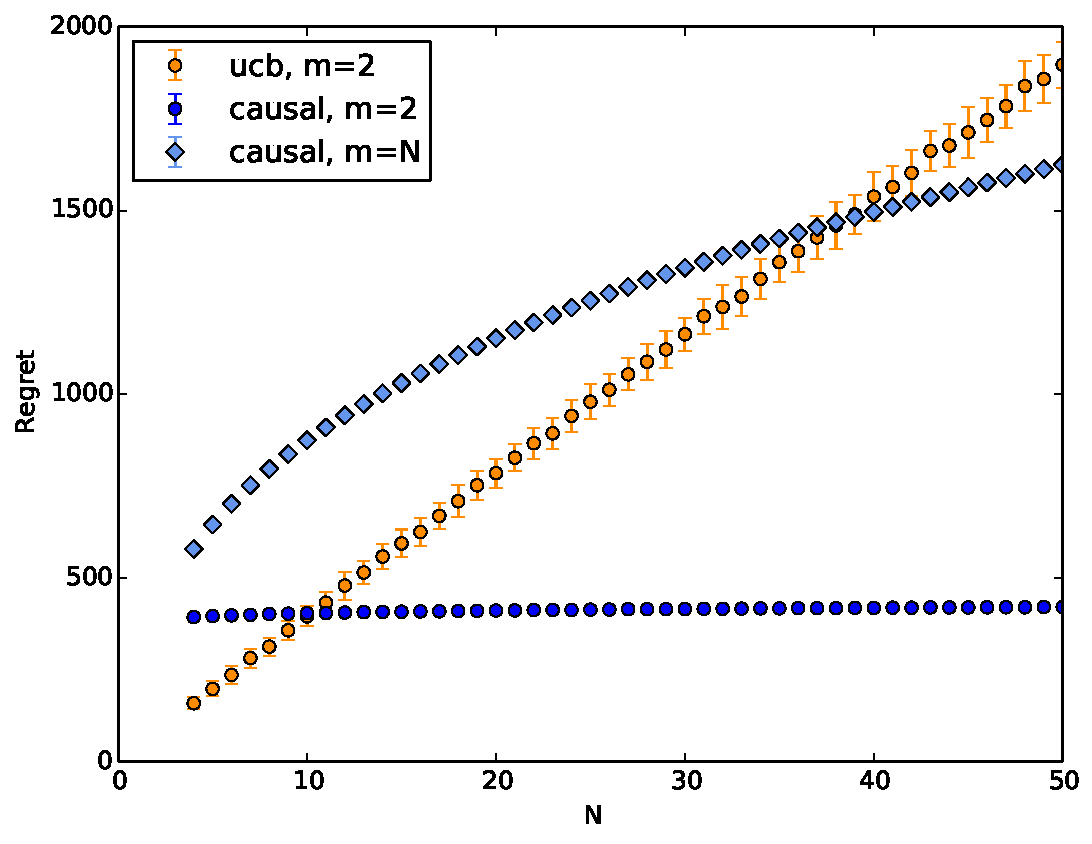
\includegraphics[width=.5\textwidth]{exp_regret_vs_N_T10000_sims100_20151229_113550.pdf}
\end{figure}

\iffalse
\begin{figure}
\caption{Cumulative regret over time for $N = 17$ for UCB with $\alpha=2$, Causal-Explore-Exploit with $m=2$ and Causal-Explore-Exploit with $m=N$. Shaded region shows standard deviation over 100 simulations. The Causal-Explore-Exploit algorithm incurs linear regret during the exploration phase, after which it selects the optimal arm with high probability. For $m=2$, we have $K \sim m^{2/3}T^{1/3}$ and see that we are in the regime in which Causal-Explore-Exploit outperforms UCB.}
\label{fig:known_q_r_vs_t}
\centering
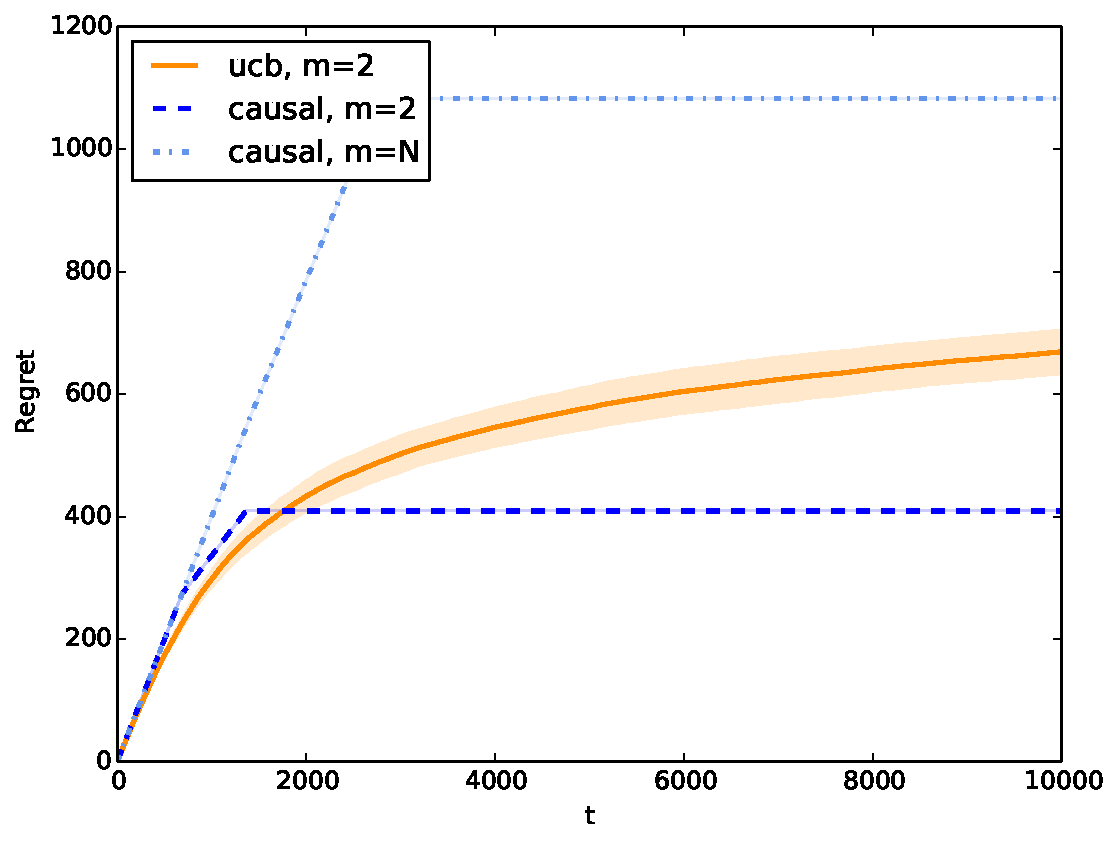
\includegraphics[width=.5\textwidth]{exp_regret_vs_t_T10000_N17_sims100_20151229_120647.pdf}
\end{figure}
\fi

\begin{figure}
\caption{Simple regret vs horizon, $T$, with $N = 20$ and fixed $\epsilon = .4$ for Successive Rejects and Causal-Best-Arm-Identification. Error bars show standard error over 100000 simulations.}
\label{fig:simple_vs_T}
\centering
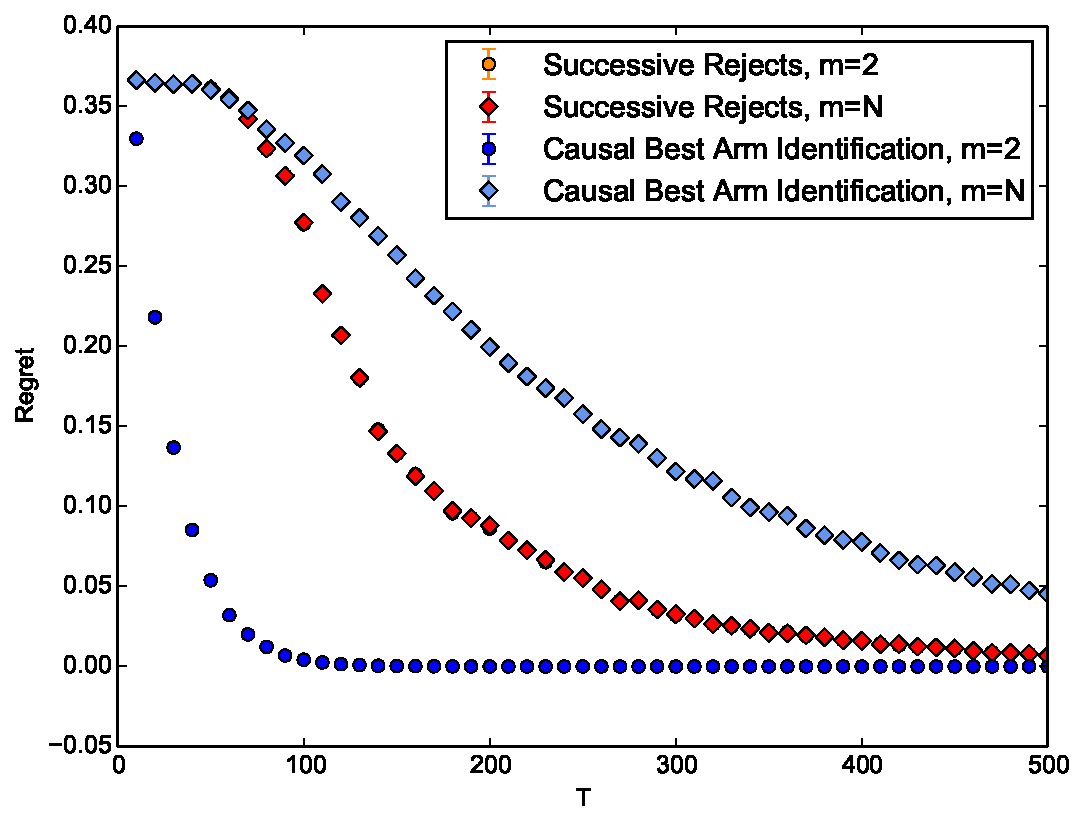
\includegraphics[width=.5\textwidth]{exp_simpleregret_vs_T_N20_sims100000_20160121_140227}
\end{figure}

\begin{figure}
\caption{Simple regret vs horizon, $T$, with $N = 20$ and $\epsilon \propto \sqrt{1/T}$ for Successive Rejects and Causal Best Arm Identification. Error bars show standard error over 10000 simulations.}
\label{fig:simple_vs_T_vary_epsilon}
\centering
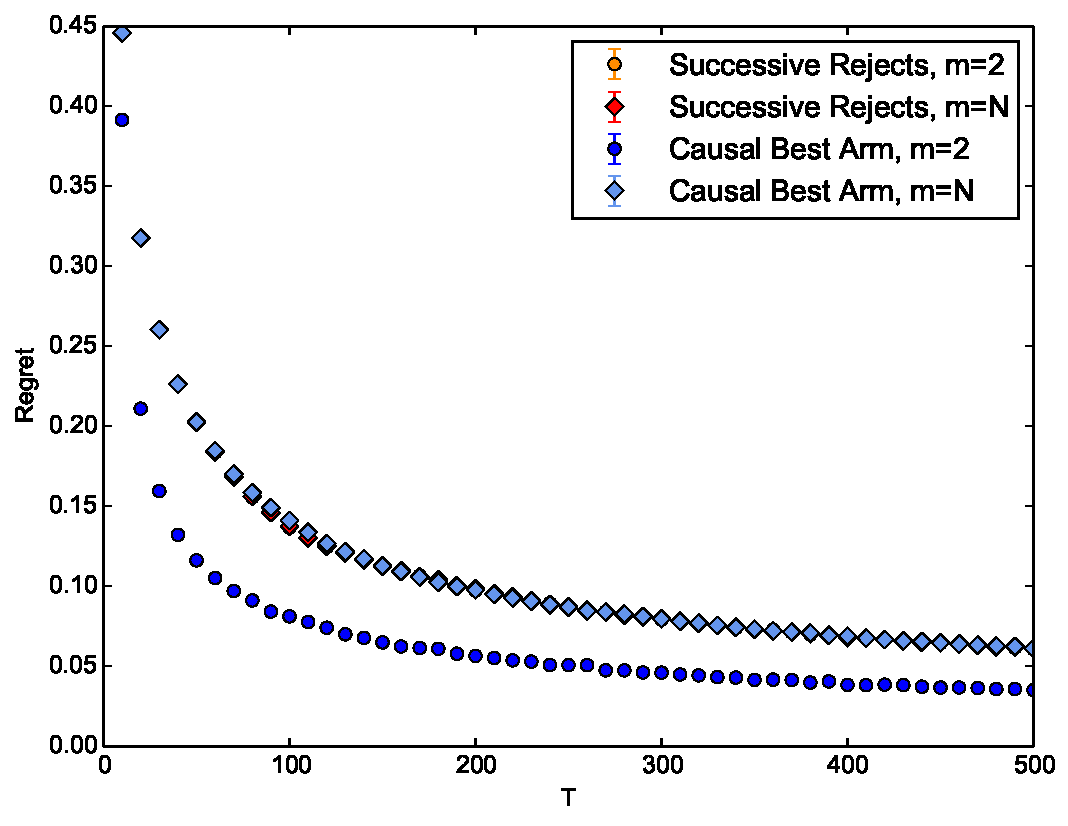
\includegraphics[width=.5\textwidth]{exp_simpleregret_vs_T_N20_sims10000_20160122_010802.pdf}
\end{figure}

\iffalse
\begin{figure}
\caption{Simple regret vs number of variables, $N$, for $T=250$, for Successive Rejects and, Causal-Best-Arm-Identification. Error bars show standard error from 10000 simulations.}
\label{fig:simple_vs_N}
\centering
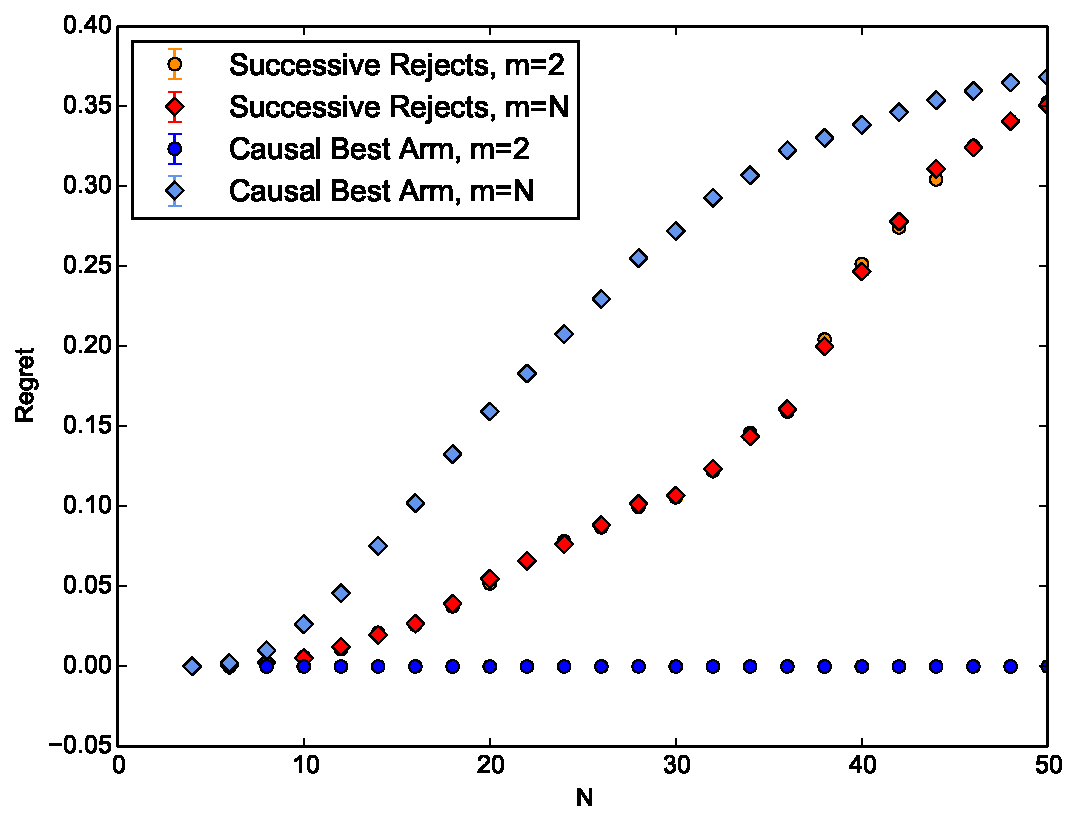
\includegraphics[width=.5\textwidth]{exp_simpleregret_vs_N_T250_sims10000_20160122_024459.pdf}
\end{figure}
\fi


\begin{figure}
\caption{Simple regret vs number of variables, $m$, for $T=300$ and $N = 50$, for Successive Rejects and Causal-Best-Arm-Identification. Error bars show standard error over 10000 simulations.}
\label{fig:simple_vs_m}
\centering
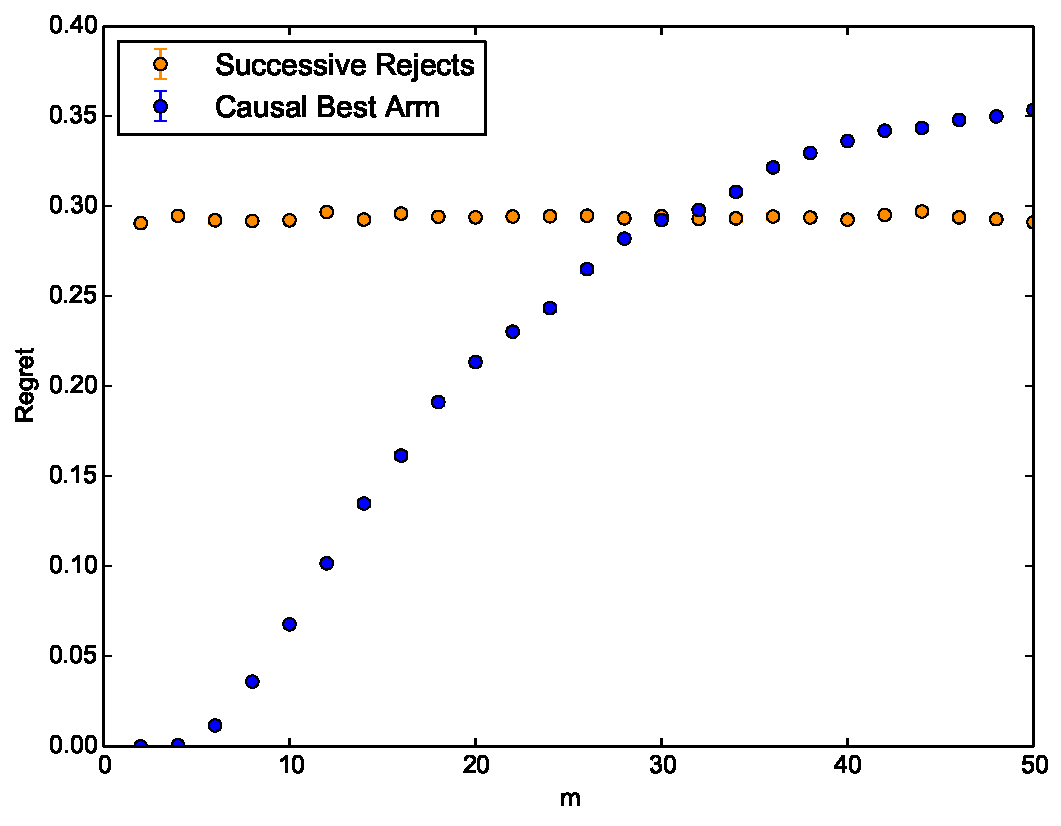
\includegraphics[width=.5\textwidth]{exp_simpleregret_vs_m_T300_N50_sims10000_10000.pdf}
\end{figure}

\iffalse
\begin{figure}
\caption{Simple regret vs number of variables, $N$, for $T=250$, for Successive Rejects and, Causal-Best-Arm-Identification on the confounded bandit problem. Error bars show standard error from 10000 simulations.}
\label{fig:simple_vs_N_confounded}
\centering
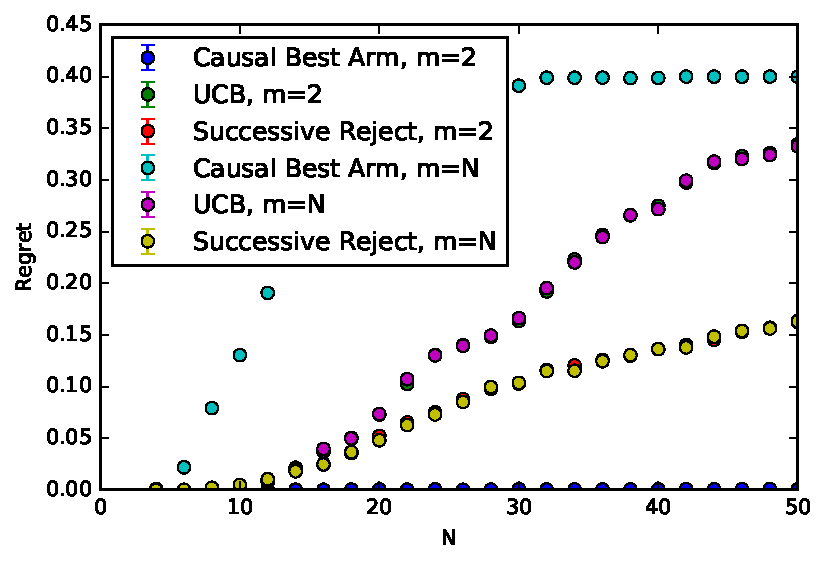
\includegraphics[width=.5\textwidth]{exp_general_simpleregret_vs_N_T250_sims10000_20160131_080208.pdf}
\end{figure}
\fi

\subsection{Experiments on more general graphs}
We now demonstrate the general simple regret algorithm on some graphs that display some interesting behaviour.
 
\begin{figure}[h]
\centering
\caption{Causal model for the confounded bandits problem.}
\label{fig:causalStructure_confounded_N}
\begin{tikzpicture}[->,>=stealth',shorten >=1pt,auto,node distance=1cm,
  thick,main node/.style={observed}, hidden/.style={empty}]
\node[main node](1){$X_{2}$};
\node[main node, right=of 1](2){$X_{3}$};
\node[hidden, right=of 2](3){$...$};
\node[main node, right=of 3](4){$X_{N}$};
\node[main node, below right=of 2](5){Y};
\node[main node,above right=of 2](6){$X_1$}; 
 \path[every node/.style={font=\sffamily\small}]
    (1) edge (5)
    	(2) edge (5)
    (4) edge (5)
    (6) edge (1) edge (2) edge (4);
\end{tikzpicture}
\end{figure}

\subsubsection{X1-dominated confounded model}
A model under which the value of the confounding variable $X_1$ plays the central role in determining $P(Y)$.  Let:
\eq {
\P{Z = 1} &= q \\
\P{X_k = 1|Z=j} &=  q_j \;\; \forall k \in \set{1...n}\\
\P{Y|x_1 ... x_n} &= \bar{\boldsymbol{x}}
} 
This leads to rewards:
\eq {
\P{Y|do(Z = j)} = q^j(1-q)^{1-j}\\
\P{Y|do(X_i = j)} = \begin{cases}
\frac{1}{n} + \frac{n-1}{n}\left(q q_1 + (1-q)q_0 \right) & \text{ if } j = 1 \\
\frac{n-1}{n}\left(q q_1 + (1-q)q_0 \right) & \text { if } j = 0
\end{cases}
}

We can select the probabilities to create a scenario close to the worst case problem such that there is a single arm $do(Z=1)$ that is optimal with expected reward ...



%%%%%%%%%%%%%%%%%%%%%%%%%%%%%%%%%%%%%%%%%%%%%%%%%
% DISCUSSION
%%%%%%%%%%%%%%%%%%%%%%%%%%%%%%%%%%%%%%%%%%%%%%%%%
\section{Discussion \& Future Work}
\label{sec:discussion}

Algorithm~\ref{alg:general} for general causal bandit problems adaptively estimates the reward for all allowable interventions $a \in \calA$ over $T$ rounds by sampling and applying interventions from a distribution $\eta$.
Theorem~\ref{thm:general} shows that this algorithm has (up to log factors) simple regret that is $\bigo{\sqrt{m(\eta)/T}}$ and that the parameter $m(\eta)$ is always less than $N$.
The value of $m(\eta)$ is a uniform bound on the variance of the reward estimators $\hat{\mu}_a$ and, intuitively, problems where all variables' values in the causal model ``occur naturally'' when interventions are sampled from $\eta$ will have low values of $m(\eta)$.

The main practical drawback of Algorithm~\ref{alg:general} is that both the estimator terms $Z_a$ and the optimal sampling distribution $\eta^*$ (\ie, the one that minimises $m(\eta)$) require knowledge of the conditional distributions $P_a$ for all $a \in \calA$.
In contrast, in the special case of parallel bandits, Algorithm~\ref{alg:simple} uses the $do()$ action to effectively estimate $m(\eta)$ and the rewards then re-samples the interventions with variances that are not bound by $\hat{m}(\eta)$.
Despite these extra estimates, Theorem~\ref{thm:lower} shows that this approach is optimal (up to log factors).
Finding an algorithm that only requires the causal graph and lower bounds for its simple regret in the general case is left as future work.

\paragraph{Cumulative Regret}
Although we have focused on simple regret in our analysis, a natural question is whether cumulative regret bounds can be obtained for the general causal bandit problem we have proposed.
% In the case of the parallel bandit problem however, we can make use of existing work on bandits with graph feedback to achieve this.

\todom{Not sure about reduction here}
Cumulative regret... use \citep{wu2015online} to get optimal cumulative regret bound (should be $\Omega(T^{2/3})$?)

General discussion of how to map parallel bandit problem to graph feedback?

% In our algorithm, we have only used the side information provided by the $do()$ action about other actions. Since the $do()$ action fully reveals the value of alternate actions we could have incorporated this information via the graph feedback model \cite{Mannor2011}, where at each timestep the feedback graph $G_t$ is selected stochastically, dependent on $\boldsymbol{q}$, and revealed after an action has been chosen. The feedback graph is distinct from the causal graph. A link $A \rightarrow B$ in $G_t$ indicates that selecting the action $A$ reveals the reward for action $B$. For this specific problem, $G_t$ will always be a star graph with the action $do()$ connected to half the remaining actions. The Exp3-IX algorithm \cite{Kocak2014} was developed for the adversarial version of this problem and has regret $\bigo{\sqrt{\bar{\alpha}T}}$, where $\bar{\alpha}$ is the average independence number of $G_t$. In our case $\bar{\alpha} = \frac{N}{2}$ so we again obtain the regret of the standard bandit algorithm. The issue here is that a malicious adversary can select the same graph each time, such that the rewards for half the arms are never revealed by the informative action. This is equivalent to a, nominally, stochastic selection of feedback graph where $\boldsymbol{q} = \boldsymbol{0}$

% \cite{Lelarge2012} consider a stochastic version of the graph feedback problem, but with a fixed graph available to the algorithm before it must select an action. In addition, their algorithm is not optimal for all graph structures and fails, in particular, to provide improvements for star like graphs as in our case. \cite{Buccapatnam2014} improve the dependence of the algorithm on the graph structure but still assume the graph is fixed and available to the algorithm before the action is selected. 

% Non-observable variables? 
% Currently assume all P_a are available (implied by observablity)
%   - do calculus' identifability
%   - non-ident variables into infinite variance case.

\paragraph{Causal Models with Non-Observable Variables}
We have assumed through this paper that all variables in the causal model were observable after an intervention is made.
A natural generalisation of our model would be for some variables to be unobservable.
\todom{More to say here?}
If the conditional models are known then the $Z_a$ terms in Algorithm~\ref{alg:general} could still be obtained via marginalising.
However, if this is not the case the estimation problem becomes more difficult.
% In this case, some conditional distributions may be non-identifiable. 
% The corresponding actions can be immediately added to the set $A$ prior to collecting any data. 
% We can then use the same algorithm as in the case where there are no latent variables, except that we will have to use the more general do-calculus rather than simply adjusting for the parents to write the expression for each action in terms of observational data.
Combining our estimation techniques with insights from \citet{Bareinboim2015} for handling unobserved confounders would be worth investigation.


% More generally, assuming causal structure creates more complex types of side information, such as that shown in equation \ref{eq:estimation_transfer}. In this case, selecting one action does not fully reveal an alternate action but provides some information towards an estimate. The quality of the estimate notably depends not only on the number of times that action was selected. For example, to get a good estimate for $X_1 = 1$ by intervening on $X_2$ requires us to sample both $X_2=0$ and $X_2=1$, in proportions dependent on $q_2$. This more complex side information does not fit within the graph feedback framework.



\paragraph{Partially or Completely Unknown Causal Graph}
A much more difficult generalisation would be to consider causal bandit problems where the causal graph is completely unknown or known to be a member of class of models.
The latter case arises naturally if we assume free access to a large observational dataset, from which the Markov equivalence class can be found via causal discovery techniques. 
Work on the problem of selecting experiments to discover the correct causal graph from within a Markov equivalence class~\cite{Eberhardt2005,eberhardt2010causal,hauser2014two,Hu2014} could potentially be incorporated into a causal bandit algorithm as part of a pre-processing step.
Simultaneously learning a completely unknown causal model while estimating the rewards of interventions would be much more challenging but there is 
\todom{Ideas? Relevant refs?}
	
% (Partially known structure)
% Key results $bigo(n)$ singleton or $bigo(log log n)$ multi-variate experiments are required.
% - Focus on minimizing the number of experiments that must be performed. Examples of active versus online learning. The cost of experiments constant or at least known. 

% (Unknown Structure)
% If we need to learn the structure, in an online environment. 
% Experiment is much, much more revealing than inference from observational data. We would expect it to dominate. 




\bibliography{libraryicml}
\bibliographystyle{icml2016}

\ifsup
\onecolumn



%%%%%%%%%%%%%%%%%%%%%%%%%%%%%%%%%%%%%%%%%%%%
% PROOF OF SIMPLE REGRET UPPER BOUND
%%%%%%%%%%%%%%%%%%%%%%%%%%%%%%%%%%%%%%%%%%%%
\section{Proof of Theorem \ref{thm:uq-simple}}\label{sec:thm:uq-simple}


Assume without loss of generality that $q_1 \leq q_2 \leq \ldots \leq q_N \leq 1/2$. The assumption is non-restrictive since all variables
are independent and permutations of the variables can be pushed to the reward function.
The proof of Theorem \ref{thm:uq-simple} requires some lemmas, the first of which is an immediate consequence of the Chernoff bound.


\begin{lemma}\label{lem:conc1}
Let $i \in \set{1,\ldots, N}$ and $\delta > 0$. Then
\eq{
\P{\left|\hat q_i - q_i\right| \geq \sqrt{\frac{6q_i}{T} \log \frac{2}{\delta}}} \leq \delta\,.
}
\end{lemma}

\begin{lemma}\label{lem:conc2}
Let $X_1,X_2\ldots,$ be a sequence of random variables with $X_i \in [0,1]$ and $\EE X_i = p$ and $\delta \in [0,1]$.
Then 
\eq{
\P{\exists t \geq n_0 : \left|\frac{1}{t} \sum_{s=1}^t X_s - p\right| \geq \sqrt{\frac{2}{n_0} \log \frac{2}{\delta}}} \leq 4\delta\,.
}
\end{lemma}

\begin{proof}
For $\delta \geq 1/4$ the result is trivial. Otherwise 
by Hoeffding's bound and the union bound:
\eq{
\P{\exists t \geq n_0 : \left|\frac{1}{t} \sum_{s=1}^t X_s - p\right| \geq \sqrt{\frac{2}{n_0} \log \frac{2}{\delta}}} 
&\leq \sum_{t = n_0}^\infty \P{\left|\frac{1}{t} \sum_{s=1}^t X_s - p\right| \geq \sqrt{\frac{2}{n_0} \log \frac{2}{\delta}}} \\
&\leq 2\sum_{t=n_0}^\infty \exp\left(-\frac{t}{n_0} \log \frac{2}{\delta}\right) 
\leq 4\delta\,. \qedhere
}
\end{proof}



\begin{lemma}\label{lem:m_est}
Let $\delta \in (0,1)$ and assume $T \geq 48m \log\frac{2N}{\delta}$. Then
\eq{
\P{2m(\vec{q}) / 3 \leq m(\vec{\hat q}) \leq 2m(\vec{q})} \geq 1 - \delta\,.
}
\end{lemma}

\begin{proof}
Let $F$ be the event that there exists and $1 \leq i \leq N$ for which
\eq{
\left|\hat q_i - q_i\right| \geq \sqrt{\frac{6q_i}{T} \log \frac{2N}{\delta}}\,.
}
Then by the union bound and Lemma \ref{lem:conc1} we have $\P{F} \leq \delta$. The result will be completed by showing that
when $F$ does not hold we have $2m(\vec{q})/3 \leq m(\vec{\hat q}) \leq 2m(\vec{q})$.
From the definition of $m(\vec{q})$ and our assumption on $\vec{q}$ we have for $i > m$ that $q_i \geq q_m \geq 1/m$ and so by Lemma \ref{lem:conc1} we have
\eq{
\frac{3}{4} 
&\geq \frac{1}{2} + \sqrt{\frac{3}{T} \log \frac{2N}{\delta}} 
\geq q_i + \sqrt{\frac{6q_i}{T} \log \frac{2N}{\delta}} 
\geq \hat q_i \\
&\geq q_i - \sqrt{\frac{6q_i}{T} \log \frac{2N}{\delta}}
\geq q_i - \sqrt{\frac{q_i}{8m}}
\geq \frac{1}{2m}\,.
}
Therefore by the pigeonhole principle we have $m(\vec{\hat q}) \leq 2m$.
For the other direction we proceed in a similar fashion. Since the failure event $F$ does not hold we have for $i \leq m$ that
\eq{
\hat q_i 
\leq q_i + \sqrt{\frac{6q_i}{T} \log\frac{2N}{\delta}} 
\leq \frac{1}{m} \left(1 + \sqrt{\frac{1}{8}}\right)
\leq \frac{3}{2m}\,.
}
Therefore $m(\vec{\hat q}) \geq 2m(\vec{q}) / 3$ as required. 
\end{proof}

\begin{proof}[Proof of Theorem \ref{thm:uq-simple}]
Let $\delta = m = m(\vec{q}) / N$. Then by Lemma \ref{lem:m_est} we have 
\eq{
\P{2m/3 \leq m(\vec{\hat q}) \leq 2m} \geq 1 - \delta\,.
}
Recall that $A = \set{a \in \actions : \hat p_a \leq 1/m(\vec{\hat q})}$. Then
for $a \in A$ the algorithm estimates $\mu_a$ from $T/(2m(\vec{\hat q})) \geq T/(4m)$ samples.
Therefore by Hoeffding's inequality and the union bound we have
\eq{
\P{\exists a \in A : |\mu_a - \hat \mu_a| \geq \sqrt{\frac{8m}{T} \log\frac{2N}{\delta}}} \leq \delta\,.
}
For arms not in $a$ we have $\hat p_a \geq 1/m(\vec{\hat q}) \geq 1/(2m)$.
Therefore if $a = do(X_i = j)$, then 
\eq{
\hat p_a = \frac{2}{T} \sum_{t=1}^{T/2} \ind{X_i = j} \geq \frac{1}{2m}\,. 
}
Therefore $\sum_{t=1}^{T/2} \ind{X_{t,i} = j} \geq T/4m$
and by Lemma \ref{lem:conc2} we have
\eq{
\P{\sum_{t=1}^{T/2} \ind{X_i = j} \geq \frac{T}{4m} \text{ and } \left|\hat \mu_a - \mu_a\right| \geq \sqrt{\frac{8m}{T} \log \frac{2N}{\delta}}} \leq 4\delta / N\,.
}
Therefore with probability at least $1 - 6\delta$ we have
\eq{
(\forall a \in \actions) \qquad |\hat \mu_a - \mu_a| \leq \sqrt{\frac{8m}{T} \log \frac{N}{\delta}} = \epsilon\,.
}
If this occurs, then 
\eq{
\mu_{\hat a^*_T} \geq \hat \mu_{\hat a^*_T} - \epsilon \geq \hat \mu_{a^*} - \epsilon \geq \mu_{a^*} - 2\epsilon\,.
}
Therefore
\eq{
\mu^* - \EE[\mu_{\hat a^*_T}] 
\leq 6\delta + \epsilon 
\leq \frac{6m}{T} + \sqrt{\frac{32m}{T} \log \frac{NT}{m}}\,, 
}
which completes the result.
\end{proof}

%%%%%%%%%%%%%%%%%%%%%%%%%%%%%%%%%%%%%%%%%%%%
% LOWER BOUND
%%%%%%%%%%%%%%%%%%%%%%%%%%%%%%%%%%%%%%%%%%%%
\section{Proof of Theorem \ref{thm:lower}}\label{sec:thm:lower}

We follow a relatively standard path by choosing multiple environments that have different optimal arms, but which cannot all be statistically
separated in $T$ rounds.
Assume without loss of generality that $q_1 \leq q_2 \leq \ldots \leq q_N \leq 1/2$.
For each $i$ define reward function $r_i$ by
\eq{
r_0(\boldsymbol{X}) &= \frac{1}{2} &
r_i(\boldsymbol{X}) &= \begin{cases}
\frac{1}{2} + \epsilon & \text{if } X_i = 1 \\
\frac{1}{2} & \text{otherwise}\,,
\end{cases}
}
where $1/4 \geq \epsilon > 0$ is some constant to be chosen later.
We abbreviate $R_{T,i}$ to be the expected simple regret incurred when interacting with the
environment determined by $\boldsymbol{q}$ and $r_i$. Let $\operatorname{P}_i$ be the corresponding measure
on all observations over all $T$ rounds and $\EE_i$ the expectation with respect to $\operatorname{P}_i$. By Lemma 2.6 by \citet{Tsy08} we have
\eq{
\Prz{\hat a^*_T = a^*} + \Pri{\hat a^*_T \neq a^*} \geq \exp\left(-\KL(\operatorname{P}_0, \operatorname{P}_i)\right)\,,
}
where $\KL(\Ps_0, \Ps_i)$ is the KL divergence between measures $\operatorname{P}_0$ and $\operatorname{P}_i$.
Let $T_i(T) = \sum_{t=1}^T \ind{a_t = do(X_i = 1)}$ be the total number of times the learner intervenes on variable $i$ by setting it to $1$.
Then for $i \leq m$ we have $q_i \leq 1/m$ and the KL divergence between $\Ps_0$ and $\Ps_i$ may be bounded using the telescoping property (chain rule) and
by bounding the local KL divergence by the $\chi$-squared distance as by \citet{Auer1995}. This leads to 
\eq{
\KL(\Ps_0, \Ps_i) 
&\leq 6\epsilon^2 \EE_0\left[\sum_{t=1}^T \ind{X_{t,i} = 1}\right] 
\leq 6\epsilon^2 \left(\EE_0 T_i(T) + q_i T\right) 
\leq 6\epsilon^2 \left(\EE_0 T_i(T) + \frac{T}{m}\right)\,.
}
Define set $A = \set{i \leq m : \EE_0 T_i(T) \leq 2T / m}$.
Then for $i \in A$ and choosing $\epsilon = \min\set{1/4, \sqrt{m/(18T)}}$ we have
\eq{
\KL(\Ps_0, \Ps_i) \leq \frac{18T\epsilon^2}{m} = 1\,. 
}
Now $\sum_{i=1}^m \EE_0 T_i(T) \leq T$, which implies that $|A| \geq m/2$.
Therefore
\eq{
\sum_{i \in A} \Pri{\hat a^*_T \neq a} 
\geq \sum_{i \in A} \exp\left(-\KL(\Ps_0, \Ps_i)\right) - 1
\geq \frac{|A|}{e} - 1 
\geq \frac{m}{2e} - 1\,.
}
Therefore there exists an $i \in A$ such that
$\Pri{\hat a^*_T \neq a^*} \geq \frac{\frac{m}{2e} - 1}{m}$. 
Therefore if $\epsilon < 1/4$ we have
\eq{
R_{T,i} \geq \frac{1}{2} \Pn{i}{\hat a^*_T \neq a^*} \epsilon \geq \frac{\frac{m}{2e} - 1}{2m} \sqrt{\frac{m}{18T}}\,.
}
Otherwise $m \geq 18T$ so $\sqrt{m/T} = \Omega(1)$ and
\eq{
R_{T,i} \geq \frac{1}{2} \Pn{i}{\hat a^*_T \neq a^*} \epsilon \geq \frac{1}{4} \frac{\frac{m}{2e} - 1}{2m} \in \Omega(1) 
}
as required.

%%%%%%%%%%%%%%%%%%%%%%%%%%%%%%%%%%%%%%%%%%%%
% GENERAL-GRAPH UPPER BOUND
%%%%%%%%%%%%%%%%%%%%%%%%%%%%%%%%%%%%%%%%%%%%
\section{Proof of Theorem \ref{thm:general}}\label{sec:thm:general}

\begin{proof}
First note that $X_t, Y_t$ are sampled from $\operatorname{Q}$.
W define $Z_a(X_t) = Y_t R_a(X_t)\ind{R_a(X_t)\leq B_a}$ and abbreviate $Z_{at} = Z_a(X_t)$ and $R_{at} = R_a(X_t)$.
By definition we have $|Z_{at}| \leq B_a$ and 
\eq{
\Var_Q[Z_{at}] 
\leq \EE_Q[Z_{at}^2] 
\leq \EEa\left[\frac{\Pn{a}{\parents{Y}(X)}}{\Q{\parents{Y}(X)}}\right] 
\leq m(\eta)\,.
}
Checking the expectation we have
\eq{
\EE_Q[Z_{at}] 
= \EEa \left[Y \ind{R_{at} \leq B_a}\right] 
= \EEa Y - \EEa \left[Y\ind{R_a > B_a}\right] 
= \mu_a - \beta_a\,,
}
where 
\eq{
0 \leq \beta_a = \EEa[Y \ind{R_a > B_a}] \leq \Pn{a}{R_a(X) > B_a}
}
is the negative bias. 
The bias may be bounded in terms of $m(\eta)$ via an application of Markov's inequality.
\eq{
\beta_a \leq \Pn{a}{R_a(X) > B_a} \leq \frac{\EEa[R_a(X)]}{B_a} \leq \frac{m(\eta)}{B_a}\,.
}
Let $\epsilon_a > 0$ be given by
\eq{
\epsilon = \sqrt{\frac{2m(\eta)}{T} \log\left(2T|\calA|\right)} + \frac{3B_a}{T} \log\left(2T|\calA|\right)\,.
}
Then by the union bound and Bernstein's inequality 
\eq{
\P{\text{exists } a \in \calA : \left|\hat \mu_a - \EE_Q[\hat \mu_a]\right| \geq \epsilon_a} 
\leq \sum_{a \in \calA} \P{\left|\hat \mu_a - \EE_Q[\hat \mu_a]\right| \geq \epsilon_a} \leq \frac{1}{T}\,.
}
Assuming this event does not occur and letting $a^* = \argmax_{a \in \calA} \mu_a$ we have
\eq{
\mu_I \geq \hat \mu_I - \epsilon_I  
\geq \hat \mu_{a^*} - \epsilon_I  
\geq \mu^* - \epsilon_{a^*} - \epsilon_I - \beta_{a^*}\,. 
}
By the definition of the truncation
we have
\eq{
\epsilon_a \leq \left(\sqrt{2} + 3\right)\sqrt{\frac{m(\eta)}{T} \log\left(2T|\calA|\right)}
}
and
\eq{
\beta_a \leq \sqrt{\frac{m(\eta)}{T} \log\left(2T|\calA|\right)}\,. 
}
Therefore for $C = \sqrt{2} + 4$ we have
\eq{
\P{\mu_I \geq \mu^* - C \sqrt{\frac{m(\eta)}{T} \log\left(2T|\calA|\right)}} \leq \frac{1}{T}\,.
}
Therefore
\eq{
\mu^* - \EE[\mu_I] \leq C \sqrt{\frac{m(\eta)}{T} \log\left(2T|\calA|\right)} + \frac{1}{T}
}
as required.
\end{proof}

\subsection{Relationship between $m(\eta)$ and $m(\boldsymbol{q})$}

\begin{proposition}\label{pro:m-equivelence} In the parallel bandit setting,
$m(\eta^*) \leq 2m(\boldsymbol{q})$.
\end{proposition} 

\begin{proof}

Recall that in the parallel bandit setting,

\eq{
\mathcal{A} = \set{do()} \cup \set{ do(X_i = j) \colon 1 \leq i \leq N \text{ and } j \in \set{0,1}}
}

Let:

\eq {
\eta_a = \ind{\P{X_i = j} < \frac{1}{m(\boldsymbol{q})}}\frac{1}{2m(\boldsymbol{q})} \text { for } a \in do(X_i = j)
}

Let $D =\sum_{a\in do(X_i=j)}\eta_a$. From the definition of $m(\boldsymbol{q})$, 
\eq {
\sum_{a\in do(X_i=j)} \ind{\P{X_i = j} < \frac{1}{m(\boldsymbol{q})}} \leq m(\boldsymbol{q}) \implies D \leq \frac{1}{2}
}
 
Let $\eta_a = \frac{1}{2} + (1-D)$ for $a = do()$ such that $\sum_{a \in \calA}\eta_a = 1$ 

Recall that,

\eq{
m(\eta) &
= \max_a \EEa\left[\frac{\Pn{a}{\parents{Y}(X)}}{\Q{\parents{Y}(X)}}\right]
}

We now show that our choice of $\eta$ ensures $\EEa\left[\frac{\Pn{a}{\parents{Y}(X)}}{\Q{\parents{Y}(X)}}\right] \leq 2m(\boldsymbol{q})$ for all actions $a$.

For the actions $a: \eta_a > 0$, ie $do()$ and $do(X_i = j):\P{X_i=j}<\frac{1}{m(\boldsymbol{q})}$,
\eq{
\EEa\left[\frac{\Pn{a}{X_1...X_N}}{\sum_{b}\eta_b\Pn{b}{X_1...X_N}}\right] \leq \EEa\left[\frac{\Pn{a}{X_1...X_N}}{\eta_a\Pn{a}{X_1...X_N}}\right] = \EEa\left[\frac{1}{\eta_a}\right] \leq 2m(\boldsymbol{q})
}

For the actions $a :\eta_a = 0$, ie $do(X_i=j):\P{X_i=j}\geq\frac{1}{m(\boldsymbol{q})}$,
\eq{
\EEa\left[\frac{\Pn{a}{X_1...X_N}}{\sum_{b}\eta_b\Pn{b}{X_1...X_N}}\right] \leq & \EEa\left[\frac{\ind{X_i=j}\prod_{k\neq i}\P{X_k}}{(1/2+D)\prod_k \P{X_k}}\right] \\=& \EEa\left[\frac{\ind{X_i=j}}{(1/2+D)\P{X_i = j}}\right]
\leq  \EEa\left[\frac{\ind{X_i=j}}{(1/2)(1/m(\boldsymbol{q}))}\right] \leq 2m(\boldsymbol{q})
}

Therefore $m(\eta*) \leq m(\eta) \leq 2m(\boldsymbol{q})$ as required.

\end{proof}
\
%in the parallel bandit setting the $m(\eta)$ given in this section approximately coincides with the $m(\vec{q})$ in Eq.\ \ref{eq:m-simple}.
%Recall in that setting that 
%\eq{
%\actions = \set{do()} \cup \set{do(X_i = j) : 1 \leq i \leq N \text{ and } j \in \set{0,1}}\,.
%}
%For $a = do()$ choose $\eta_a = 1/2$. 
%Let $m = m(\vec{q})$ and note that, by definition, there are at most $m$ pairs $(i,j)$ such that $\P{X_i = j} \leq 1/m$.
%Thus, for $a = do(X_i = j)$ letting $\eta_a \propto \ind{\P{X_i = j} \leq 1/m} / (2m)$ guarantees $\eta_a \ge \frac{1}{2m}$ when $\eta_a \ne 0$.
%It is then easy to check that $m(\eta) \leq 2m$ using an argument like that for Proposition~\ref{pro:m-bound}.



\fi


\end{document}
